% 52 weeks ahead (planned 13 November 2026, docs/PAPER1_REVISION_PLAN.md). A subsection of the results in the
% arXiv version, a section of the supplement in the journal version. Every number from
% scripts/make_long_horizon_tables.py (generated/lh_values.tex, lh_tab.tex, lh_tab_all.tex).
\ifsupplement\section{Forecasting 52 weeks ahead}\else\subsection{Forecasting 52 weeks ahead}\fi
\label{sec:long-horizon}

\textbf{Over 52 weeks the world model alone is not the most accurate forecast on
any data set. The average of the two models, each forecasting all 52 weeks at
once, is the most accurate on \lhLowestAvgDirect{} of \lhSets{} data sets, and
LightGBM on the others.} Grocery retailers plan the year ahead, so the test asks
whether the rule of Section~\ref{sec:rq-broad} carries from 8 weeks to 52. It
was written down before it ran: the six Dominick's categories and M5, two
windows of 52 weeks each (364 days on M5), the final tuned settings with only the
distance ahead changed, scored at every level as in the rest of the paper
(Table~\ref{tab:long-horizon}, Figure~\ref{fig:long-horizon}).

\paragraph{The planned comparison, in blocks}
Each model forecasts 13 weeks, takes its forecast in as the sales of those weeks,
and forecasts the next 13, four times. Here the world model is clearly less
accurate than LightGBM in \lhPWmWorse{} of \lhPN{} paired comparisons and clearly
more accurate in \lhPWmBetter{}; against the better of LightGBM's two setups it
is behind on \lhLgbBestBeatsWm{} of \lhSets{} data sets. The average in blocks is
clearly more accurate than the world model alone in \lhPAvgWmBetter{} comparisons
(clearly less in \lhPAvgWmWorse{}), and than LightGBM in \lhPAvgLgbBetter{}
(clearly less in \lhPAvgLgbWorse{}).

\paragraph{Taking in its own forecasts costs the world model most}
Forecasting all 52 weeks at once, the world model is more accurate than in blocks
on \lhDirectBeatsBlocksWm{} of \lhDirectSetsWm{} data sets, LightGBM on
\lhDirectBeatsBlocksLgb{} of \lhDirectSetsLgb{}. In blocks, the world model's item
by store error changes by \lhGrowWmLo{} to \lhGrowWmHi{} from the first 13 weeks
to the last, LightGBM's by \lhGrowLgbLo{} to \lhGrowLgbHi{}. The world model rolls
its state forward from the sales it takes in; when those are its own forecasts,
its errors are carried into the state and grow with each block.

\paragraph{The rule carries to 52 weeks}
The average of the two models, each forecasting the whole year at once, is
clearly more accurate than LightGBM forecasting directly in \lhPAvgDirBetter{} of
\lhPAvgDirN{} paired comparisons and clearly less in \lhPAvgDirWorse{}; against
the world model forecasting directly it is clearly more accurate in
\lhPAvgDirWmBetter{} and clearly less in \lhPAvgDirWmWorse{}. These two
comparisons were added after the planned ones.

\paragraph{Added after the planned test: other designs and other models}
After seeing the planned result we added two designs in which no model takes in
its own forecasts, and ran the other models of the paper over 52 weeks
(Table~\ref{tab:long-horizon-all}). In the first, the world model rolls its
state forward 13 weeks at a time on the plan; in the second, LightGBM fits one
model per block of 13 weeks. Rolling on helps on M5 and fails on Dominick's. On M5
the world model rolled on scores \lhMfiveWmRollon{} against \lhMfiveWmBlocks{} in
blocks, and its average with LightGBM, \lhMfiveAvgRollon, is the most accurate
forecast on M5 and clearly more accurate than LightGBM forecasting directly
(\lhMfiveLgbDirect) in \lhMfiveAvgRollonLgbBetter{} of
\lhMfiveAvgRollonLgbN{} paired comparisons, clearly less in none. On the
Dominick's categories the rolled-on state drifts: on cheese the forecast is
\lhRollonCheeseFa{} times what sold and the WRMSSE \lhRollonCheese. LightGBM by
block is close to LightGBM forecasting directly. Of all the forecasts, the
average with each model forecasting directly is the most accurate on
\lhAllLowestAvgDirect{} data sets, LightGBM directly or by block on two, and the
average with the world model rolled on on M5; no other model is the most
accurate anywhere. TFT, TimesFM, Chronos and the seasonal naive forecast are
behind LightGBM and the average on every data set; TimesFM given the plan is
ahead of the world model alone on analgesics. Timestral given the plan cannot
forecast 52 weeks: its forecast is \lhTimestralFaOneLo{} to \lhTimestralFaOneHi{}
times what sold in the first 13 weeks and \lhTimestralFaLo{} to
\lhTimestralFaHi{} times over the year. M5's world model forecasting all 52 weeks
at once and TFT on M5 were not run.

\begin{table*}[t]
\centering\footnotesize\setlength{\tabcolsep}{3pt}
\caption{Every forecast 52 weeks ahead (364 days on M5): WRMSSE over the 52 weeks, mean over levels and two windows.
Each forecasts all 52 weeks at once except the world model rolled on (its state rolled 13 weeks at a time on the plan,
without taking in its own forecasts) and LightGBM by block (one model per block of 13 weeks). Averages: the world
model with LightGBM directly (Avg) or by block. Tuned: settings searched again for 52 weeks on Dominick's. Bold: lowest
of each row, leaving out Timestral with the plan, which could not forecast 52 weeks. Of these, only WM, LGB and Avg
were in the planned test; the rest were added after it ran.}
\label{tab:long-horizon-all}
\begin{adjustbox}{max width=\textwidth}\begin{tabular}{lccc}
\toprule
Data set & \rotatebox{90}{WM} & \rotatebox{90}{LGB} & \rotatebox{90}{Avg}\\
\midrule
Analgesics & 0.964 & \textbf{0.867} & 0.868 \\
Bottled juice & 0.764 & 0.769 & \textbf{0.726} \\
Cheese & 0.773 & 0.707 & \textbf{0.677} \\
Frozen entrees & 0.412 & 0.393 & \textbf{0.387} \\
Soft drinks & 0.851 & \textbf{0.754} & 0.767 \\
Snacks & 0.866 & 0.882 & \textbf{0.843} \\
M5 & n/a & \textbf{0.839} & n/a \\
\bottomrule
\end{tabular}\end{adjustbox}
\end{table*}


\begin{table*}[t]
\centering\footnotesize\setlength{\tabcolsep}{3pt}
\caption{Forecasts 52 weeks ahead (364 days on M5). WRMSSE over the 52 weeks, mean over levels and two windows, for
the world model (WM), LightGBM (LGB) and their average (Avg). In blocks: each model forecasts four blocks of 13 weeks,
each block's forecast taken in as sales before the next. Direct: each model forecasts all 52 weeks at once (not run for
M5's world model). Paired item bootstrap over levels and windows: comparisons clearly lower / clearly higher, of all.
Last four columns: WRMSSE item by store in the first and last block of 13 weeks, in blocks. Shading marks the lowest
of the six: \colorbox{wmcell}{world model}, \colorbox{lgbcell}{LightGBM}, \colorbox{avgcell}{average}.}
\label{tab:long-horizon}
\begin{adjustbox}{max width=\textwidth}\begin{tabular}{l ccc ccc cc cc cc}
\toprule
 & \multicolumn{3}{c}{In blocks} & \multicolumn{3}{c}{Direct} & \multicolumn{2}{c}{Paired} & \multicolumn{2}{c}{WM, item by store} & \multicolumn{2}{c}{LGB, item by store}\\
\cmidrule(lr){2-4}\cmidrule(lr){5-7}\cmidrule(lr){8-9}\cmidrule(lr){10-11}\cmidrule(lr){12-13}
Data set & WM & LGB & Avg & WM & LGB & Avg & WM vs LGB, blocks & Avg vs LGB, direct & Weeks 1 to 13 & 40 to 52 & Weeks 1 to 13 & 40 to 52\\
\midrule
Analgesics & 1.062 & \cellcolor{lgbcell}\textbf{0.865} & 0.907 & 0.964 & 0.867 & 0.868 & 0 / 3 of 8 & 1 / 0 of 8 & 0.697 & 0.686 & 0.696 & 0.683 \\
Bottled juice & 0.903 & 0.797 & 0.817 & 0.764 & 0.769 & \cellcolor{avgcell}\textbf{0.726} & 0 / 2 of 8 & 4 / 0 of 8 & 0.738 & 0.742 & 0.705 & 0.689 \\
Cheese & 1.086 & 0.689 & 0.820 & 0.773 & 0.707 & \cellcolor{avgcell}\textbf{0.677} & 0 / 8 of 8 & 2 / 0 of 8 & 0.701 & 0.938 & 0.692 & 0.738 \\
Frozen entrees & 0.424 & 0.397 & 0.393 & 0.412 & 0.393 & \cellcolor{avgcell}\textbf{0.387} & 0 / 5 of 8 & 2 / 0 of 8 & 0.469 & 0.404 & 0.450 & 0.370 \\
Soft drinks & 0.872 & 0.862 & 0.819 & 0.851 & \cellcolor{lgbcell}\textbf{0.754} & 0.767 & 1 / 0 of 8 & 0 / 2 of 8 & 0.618 & 0.767 & 0.631 & 0.781 \\
Snacks & 1.013 & 0.877 & 0.920 & 0.866 & 0.882 & \cellcolor{avgcell}\textbf{0.843} & 0 / 6 of 8 & 6 / 0 of 8 & 0.691 & 0.890 & 0.622 & 0.683 \\
M5 & 1.016 & 0.931 & 0.874 & n/a & \cellcolor{lgbcell}\textbf{0.839} & n/a & 4 / 14 of 24 & n/a & 0.823 & 1.000 & 0.849 & 0.908 \\
\bottomrule
\end{tabular}\end{adjustbox}
\end{table*}


\begin{figure*}[t]
\centering
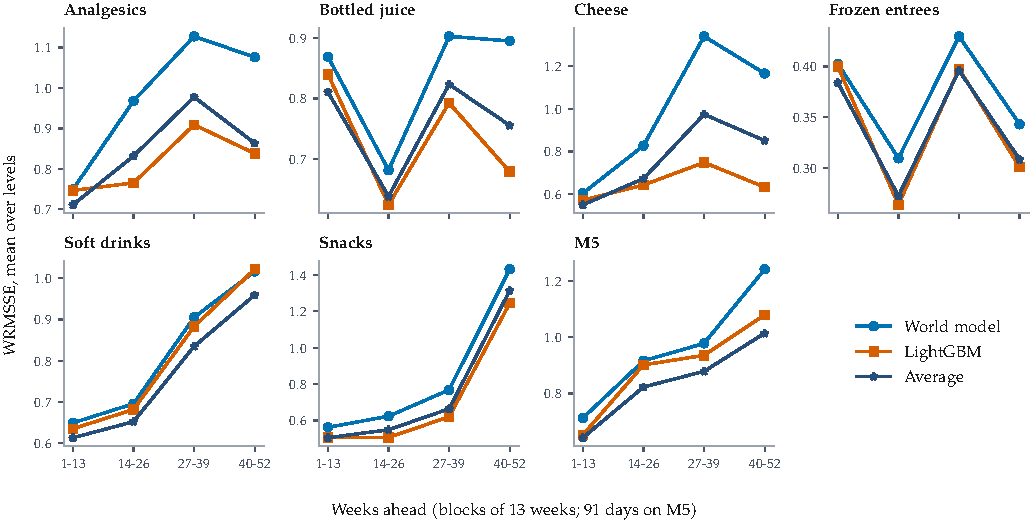
\includegraphics[width=\textwidth]{figs/fig_long_horizon.pdf}
\caption{\textbf{Taking in its own forecasts, the world model's error grows from
block to block.} WRMSSE, mean over levels and two windows, in each block of 13
weeks (91 days on M5), for the world model, LightGBM and their average
forecasting in blocks.}
\label{fig:long-horizon}
\end{figure*}
